\def\fig#1{Fig.~\ref{#1}}

% Final version: use times!
\documentclass{sig-alternate}
%\usepackage{graphicx}
%\usepackage{times}
% \draftfalse




% \documentstyle[times,graphicx,uist,isolatin1]{article}
\begin{document}

\newcommand{\url}[1]{\textsf{#1}}
\newcommand{\hyp}{\discretionary{}{}{}}


\title{
Freenet-like GUIDs for Implementing Xanalogical Hypertext
}

%%
%% Note on formatting authors at different institutions, as shown below:
%% Change width arg (currently 7cm) to parbox commands as needed to
%% accommodate widest lines, taking care not to overflow the 17.8cm line width.
%% Add or delete parboxes for additional authors at different institutions. 
%% If additional authors won't fit in one row, you can add a "\\"  at the
%% end of a parbox's closing "}" to have the next parbox start a new row.
%% Be sure NOT to put any blank lines between parbox commands!
%%
\numberofauthors{2}

\author{
\alignauthor 
    Tuomas J. Lukka\\
    \affaddr{Hyperstructure Group}\\
    \affaddr{Dept.~of Mathematical Information Technology}\\
    \affaddr{University of Jyv\"askyl\"a, PO.~Box~35}\\
    \affaddr{FIN-40351~Jyv\"askyl\"a}\\
    \affaddr{Finland}\\
    \email{lukka@iki.fi}
\alignauthor
	 Benja Fallenstein\\
    \affaddr{Oberstufen-Kolleg}\\
    \affaddr{University of Bielefeld, PO.~Box~100131}\\
    \affaddr{D-33501 Bielefeld}\\
    \affaddr{Germany}\\
    \email{b.fallenstein@gmx.de}
}

\maketitle

% \textwidth 3.5in
% \columnwidth 3.5in

\begin{abstract}

We discuss the use of Freenet-like content hash GUIDs as a primitive
for implementing the Xanadu model in a peer-to-peer framework.

Our current prototype is able to display
the implicit connection (transclusion) between
two different references to the same permanent ID.

We discuss the next layers required in
the implementation
of the Xanadu model on
a world-wide peer-to-peer network.

\end{abstract}


% \tolerance=400 
% \tolerance=500 
  % makes some lines with lots of white space, but      
  % tends to prevent words from sticking out in the margin

\def\diff{{\tt diff}}

\def\unfin{\tiny}
\def\fin{\normalsize}


\section{Introduction}

(Non-)Permanence of content is a growing problem
on the Internet, and various attempts have been made to 
alleviate it\cite{waybackmachine,simonson-content-permanence,freenet-ieee}.

The Xanadu hypermedia 
model\cite{ted-xu-vision,ted-xu-model,ted-xanalogical-structure-needed}
handles the problem by 
assigning a permanent ID to content when it first 
enters the system.
The immutable, permanent ID relates to the \emph{physical act} 
of entering the smallest units of data,
as in ``the character 'D' typed by Janne Kujala on 10/8/97 8:37:18''.
Mutable documents are represented as \emph{virtual files} containing
lists of permanent media IDs.
Copying content from one document to another is done by referring
to the same permanent IDs. 

In the Xanadu model, 
all virtual files containing a given piece
of content (\emph{transclusion}) can be found and displayed to the user.
For example, an email quoting another email would be 
automatically and implicitly connected
to the original via the transclusion.
Bidirectional, non-breaking external links 
(\emph{content linking}) can be resolved
through the same mechanism.
Nelson\cite{ted-xanalogical-structure-needed} argues that conventional
software, unable to reflect such interconnectivity of documents, is
unsuited to most human thinking and creative work.

In order to implement the Xanadu model, it must be possible to 
efficiently search for references to permanent IDs on a large
scale.
The original Xanadu design organized
content~IDs in a DNS-like hierarchical structure (tumblers), making content
references arbitrary intervals (spans) in the hierarchy. 
Advanced
tree-like data structures\cite{ted-xu-tech} were used to retrieve the content
efficiently.
Unfortunately,
Project Xanadu's implementation was never finished
and it is unclear whether the tumbler model can be implemented
securely to avoid e.g.~spoofing attacks.

In this article, we discuss a less ambitious structure
based on Freenet-like GUIDs.
This allows
distributed hashing\cite{ratnasamy00scalable,stoica01chord}
to be used for looking up references to permanent IDs.

% for searching.
% 
% There have been significant advances in the field of distributed
% indexing, keyword indexing and searching recently.
% CAN\cite{ratnasamy00scalable} (content-addressable networks) and 
% Chord\cite{stoica01chord} are
% architectures for distributed hashtables, hashing keys
% and assigning each node on the network a range of the possible
% hash values. Ideally, only the requesting node and the node
% holding that range of hash values need to be involved in a lookup.
% 
% Unfortunately, intervals like Project Xanadu's content references 
% cannot be keys in hashtable-like structures.




\section{Freenet: Globally Unique IDs}

Freenet\cite{freenet,freenet-ieee} is a decentralized peer-to-peer architecture
for anonymous uncensorable publishing.
Data is stored in immutable sequences of bytes, identified
by SHA-1 cryptographic hashes\cite{fips-sha-1} of their contents. 
Since in practice
SHA-1 hashes are unique, they can be assigned as Globally Unique IDs
(GUIDs) without needing a central naming authority.
% As a byte sequence is referred to through a
% cryptographic GUID, it does not matter that the content is obtained 
% from an untrusted source.

GUIDs are like Uniform Resource Names\cite{rfc1737}: 
they do not specify a physical
storage location but an \emph{identity}. 
In such a system, the primitive operation is \emph{not} ``get me file X
from location Y'' but ``get me the data X, whereever it may be''.
% The physical storage
% and network connections are the responsibility of the lowest layer.

\section{Xanadu-model hypertext on top of Freenet-like GUIDs}

While Freenet focuses on
anonymity and uncensorability,
Xanadu focuses on 
external linking, implicit connections via transclusions, and
permanence.
Despite the differences, 
Freenet-like GUIDs provide a useful lowest layer of abstraction
for implementing the Xanadu model.

In this model, a block of media content (e.g.~keystrokes) 
obtains a GUID when first saved to permanent storage. 
%Unlike in Freenet,
The byte sequence also contains metadata such as the author
and the creation time.
All documents referring to
the saved keystrokes use the GUID and
an offset inside the block.

With GUIDs, searching for the references can be implemented through
distributed hashtables\cite{ratnasamy00scalable,stoica01chord}, 
mapping a block's GUID to a list of references
to that block. (Tumblers, being intervals, could not be used
as hashtable keys.)

One of the advantages of using permanent blocks with GUIDs as 
a primitive is robustness. 
If a conventional application crashes while saving a file, the whole
file can get mangled. 
In our design, 
blocks with GUIDs are used to emulate append-only storage such as CD-R.
Only the difference between the
previous and the current version is stored in a new permanent block.
Even if the software crashes, the older blocks will not be harmed.

% To overcome these deficiencies, we propose to use Freenet-like 
% location-independent GUIDs [cf Freenet project, IEEE article]
% (globally unique IDs).

% Unlike Freenet, IDs are
% assigned when content first enters in the system, not when
% it is published on the network. Whereever a piece of content is used,
% it will be referenced by the same ID, so the ID will be permanent, too.
% (This makes it even more important to be able to create IDs without
% a central naming authority, so that content can be entered in a computer
% system without the system having previously been connected to a central
% naming authority.) [Previous sentence is here to remember the idea, not to
% make its way into the article.]

% Explain scrollblocks!!! Sequential keystrokes.


\begin{figure}
\centering
% 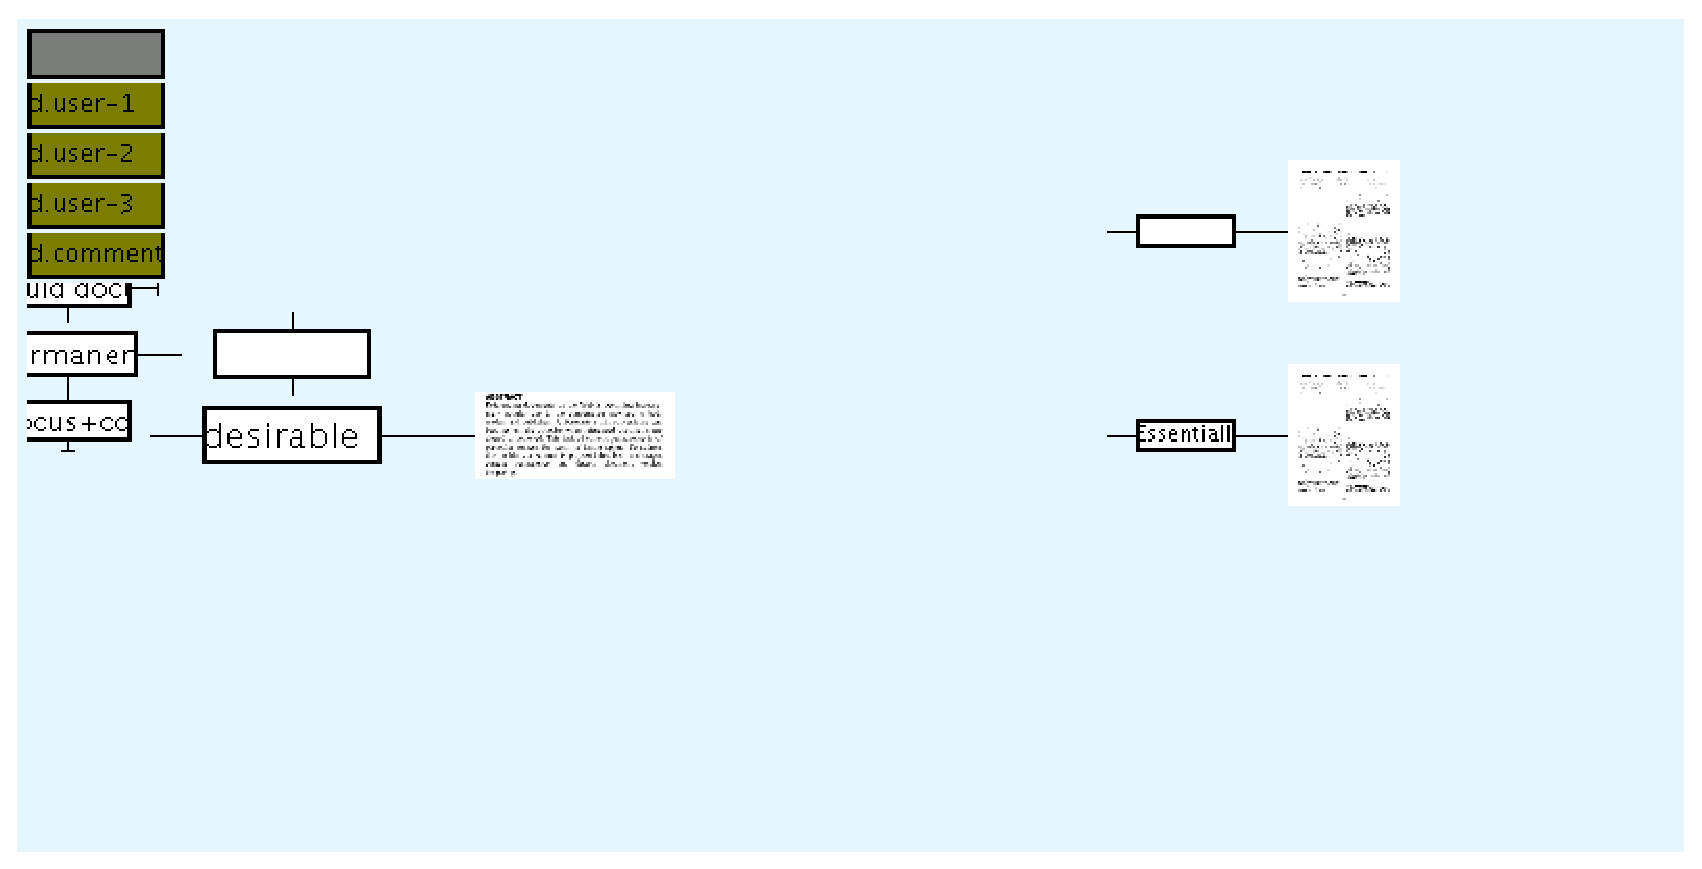
\epsfig{file=transcl.ps, height=2in, width=5in}
a)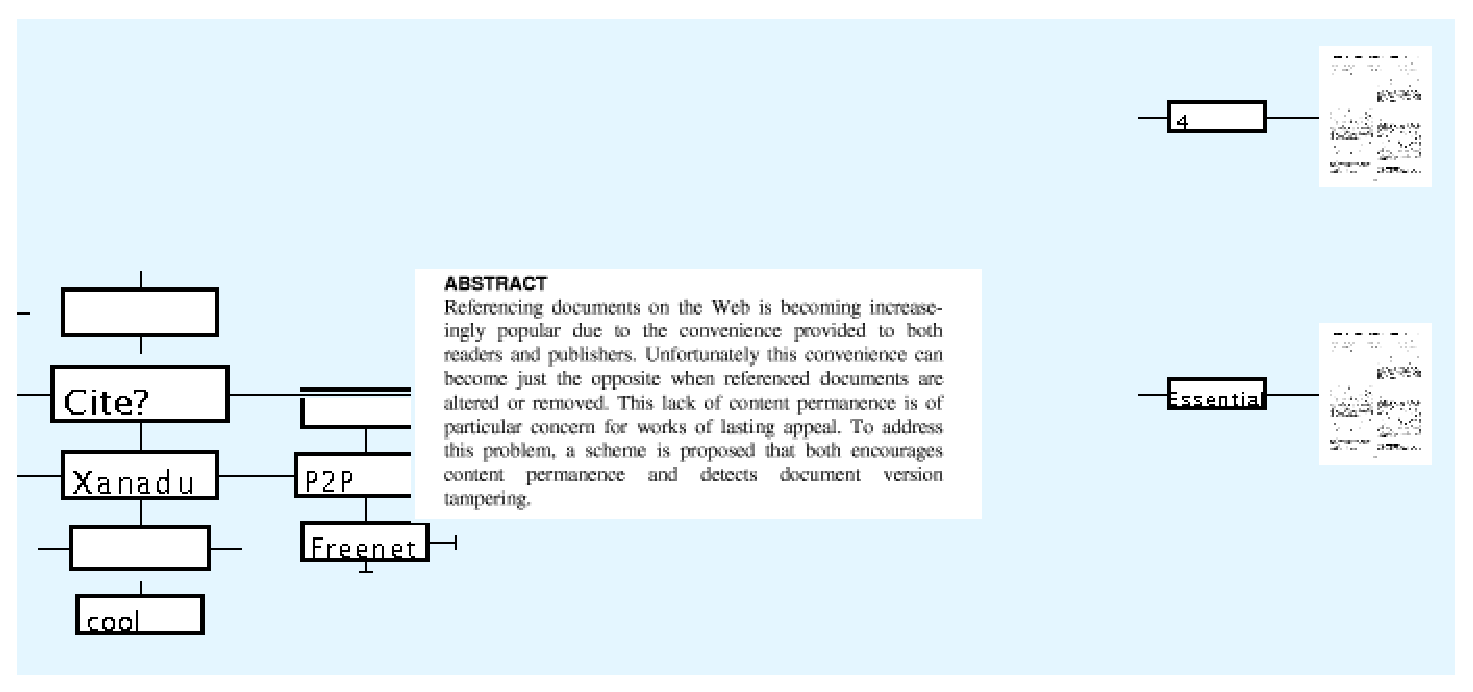
\epsfig{file=fig-a.ps, width=3.1in}
b)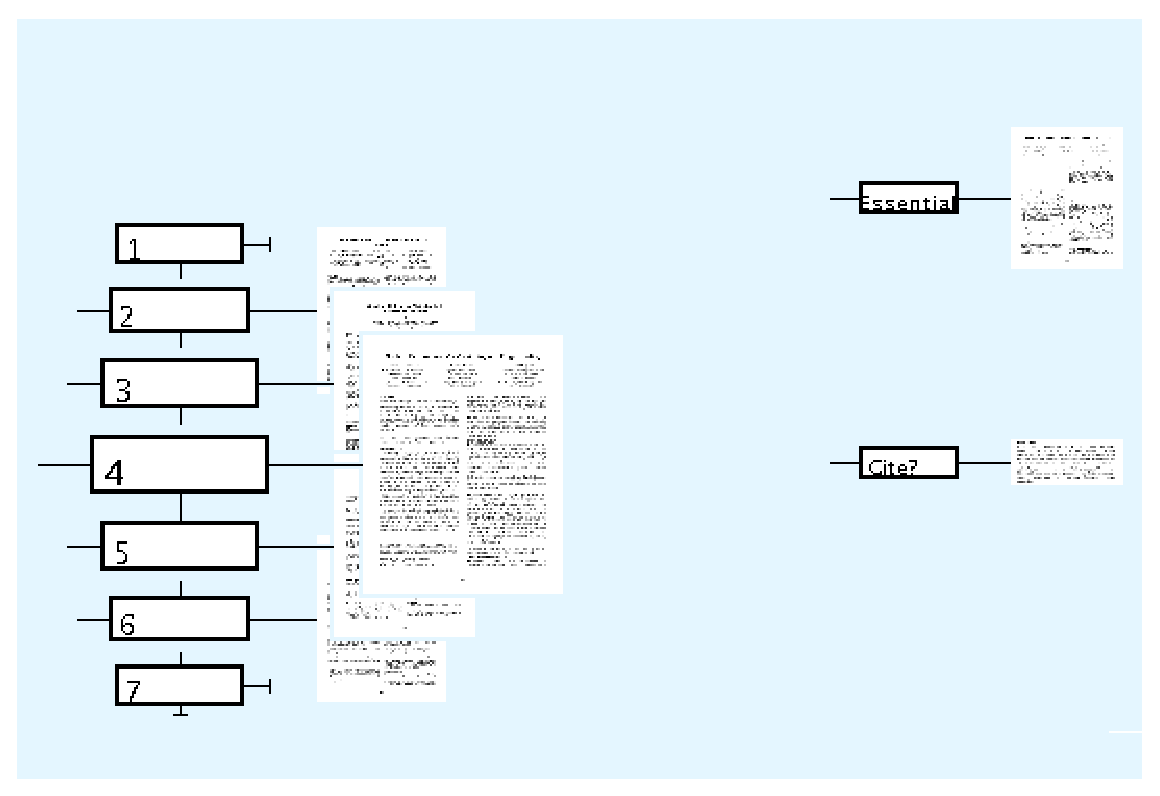
\epsfig{file=fig-b.ps, width=3.1in}
\caption{
Two screenshots
of Gzz:
a) Three trans\-clusions from an article and cells
connected to each transclusion. b) After moving the focus to another one 
of the transclusions in a) and zooming out.
(The images have been edited to fit the page.)
\label{fig-pdftrans}}
\end{figure}
\break
The block-level granularity can cause complications when
publishing a block:
if it contains something that the user does not want to distribute,
they must either create a
new, Bowdlerized block and refer to that,
or make a \emph{surrogate} block
containing the publishable parts and their permanent IDs.
Trust that a surrogate block contains the correct contents for an ID
depends on digital signatures and requires a public key infrastructure.
Checking the cryptographic hash is not possible, as only part of the
original block is available.
Being able to assign secure, permanent
identities to the individual letters would
solve this problem, but there is no known way to do this efficiently.


\section{The Gzz implementation}

The Gzz prototype\cite{gzz} uses immutable byte sequences with GUIDs 
for all permanent data. While the prototype
is not yet able to operate on a world-wide
P2P network, 
low-level synchronization among users can be performed without a central
server by simply copying the blocks.

Figure~\ref{fig-pdftrans} shows 
two screenshots of an
annotated bibliography of hypertext publications.
The focus+context\cite{fc-fisheye} view
shows two things as the context of a transclusion from a PDF file:
users' annotations, which have explicitly been connected to it; and
different transclusions of the same content, only implicitly connected
to the focused transclusion through the Xanadu model.

This functionality is currently in a pre-alpha stage, but we 
expect to release
a first version of it as a part of Gzz~0.8.0 (\emph{``chartreuse''}) shortly.




%In the figure, we see parts of an article transcluded in Gzz cells.
%Different Gzz structures are connected to each of those cells. However,
%the different transclusions from the article are not connected in Gzz
%themselves. They are shown together only because the system has
%detected they share the same content ID. (argh)

%Our prototype detects 
%transclusions between different ``documents'' open at the same
%time. Figure \ref{fig-pdftrans} shows transclusions from PDF files, allowing
%a group of users to comment on the contents of these files. 

%A user transcludes part of a PDF file into a Gzz cell, then connects
%commentary to that cell. When the user moves near a cell containing
%part of a PDF file, other cells containing an overlapping part are
%shown in the margins [fig.1]. This is an application the focus+context
%paradigm Gzz is based on: transclusions of overlapping parts from the
%same PDF file are shown as context; by clicking on them, the user
%can make them the focus, putting the formerly focused cell into the context.

%There is no explicit connection between these cells. They are only
%shown together because the system noticed they contain overlapping
%parts of the same PDF file.


\break
\section{Conclusions}

We have shown how a subset of the Xanadu media model can be implemented
using Freenet-like GUIDs.
Our current prototype is still limited:
to approach the full functionality of the Xanadu model, content links
have to be implemented, and the system
needs to be extended to 1) fetch data interactively through a P2P
network, and 2) use distributed indices of references to permanent IDs.

In addition to the implementation of the Xanadu model,
more research is needed on visualizing and navigating the structures
arising from it.

% Everyday use of the prototype 
% 
% To our knowledge it has never been in everyday
% use, 
% from actual everyday use of the Xanadu model; the 
% it seems impossible
% to predict 


% \bibliographystyle{abbrv}
\bibliographystyle{abbrv}
\bibliography{gzigzag}

\end{document}
